\subsection{Matching}

Teknikken baseret på matching repræsentere hver klasse med en \textit{prototype pattern vector}. Når der så kommer en ny ''ukendt'' vector, som skal klassifiseres bliver denne tillagt den klasse som den ligger nærmest i forhold til sin vector. Se Figur~\ref{fig:decision-boundary} hvor den sorte firkant og cirkel er ''the mean'' vectors.

\begin{figure}[h]
	\centering
	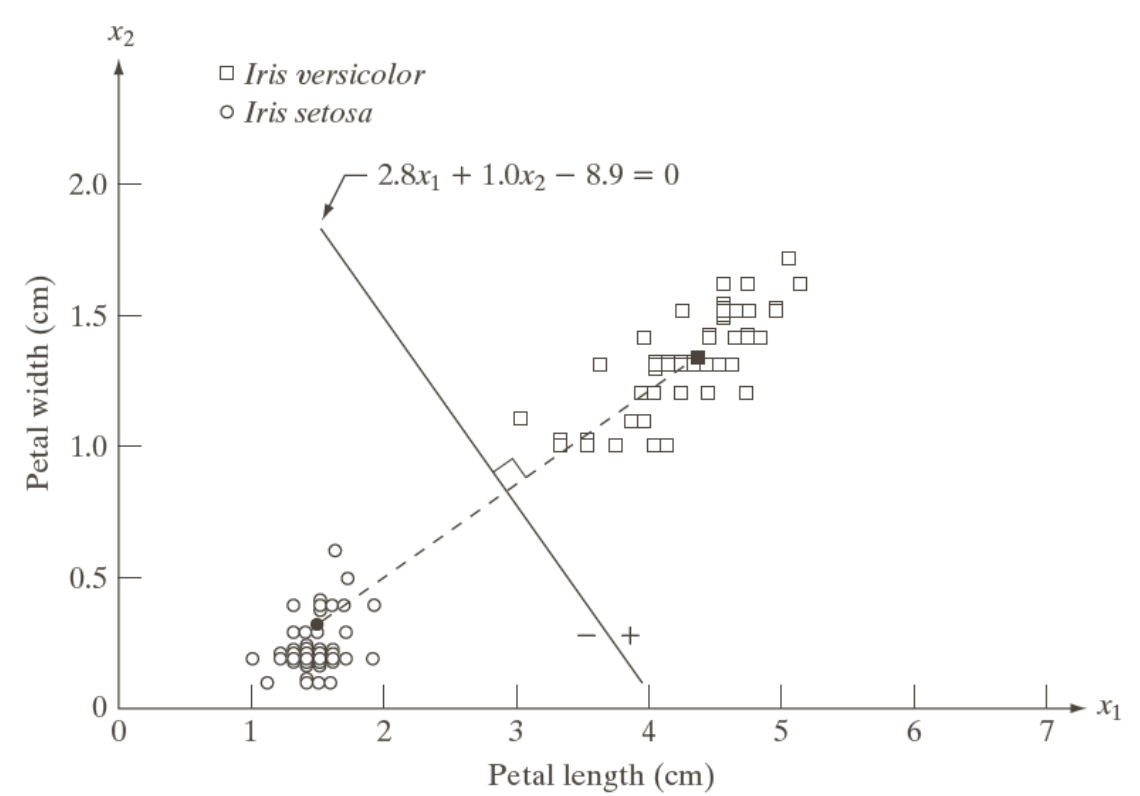
\includegraphics[width=0.9\linewidth]{figs/spm12/decision-boundary}
	\caption{Decision boundary of minimum distance classifier.}
	\label{fig:decision-boundary}
\end{figure}

\subsubsection{Minimum Distance Classifier}

Hvis vi sætter prototype vektoren til at være gennemsnittet af vektore af en klasse. Så kan vi tage den nye ''ukendte'' vektor og klassifisere den som prototype vektoren som den er tættest på.\\

Denne model virker godt hvis afstanden fra mellem de forskellige gennemsnit er stor og allerbedst når fordelingen af hver klasse omkring dens gennemsnit er i formen af en sphere ''hypercloud'' i et $n$-dimentionelt rum.
